% Options for packages loaded elsewhere
\PassOptionsToPackage{unicode}{hyperref}
\PassOptionsToPackage{hyphens}{url}
\PassOptionsToPackage{dvipsnames,svgnames*,x11names*}{xcolor}
%
\documentclass[
]{article}
\usepackage{lmodern}
\usepackage{amssymb,amsmath}
\usepackage{ifxetex,ifluatex}
\ifnum 0\ifxetex 1\fi\ifluatex 1\fi=0 % if pdftex
  \usepackage[T1]{fontenc}
  \usepackage[utf8]{inputenc}
  \usepackage{textcomp} % provide euro and other symbols
\else % if luatex or xetex
  \usepackage{unicode-math}
  \defaultfontfeatures{Scale=MatchLowercase}
  \defaultfontfeatures[\rmfamily]{Ligatures=TeX,Scale=1}
\fi
% Use upquote if available, for straight quotes in verbatim environments
\IfFileExists{upquote.sty}{\usepackage{upquote}}{}
\IfFileExists{microtype.sty}{% use microtype if available
  \usepackage[]{microtype}
  \UseMicrotypeSet[protrusion]{basicmath} % disable protrusion for tt fonts
}{}
\makeatletter
\@ifundefined{KOMAClassName}{% if non-KOMA class
  \IfFileExists{parskip.sty}{%
    \usepackage{parskip}
  }{% else
    \setlength{\parindent}{0pt}
    \setlength{\parskip}{6pt plus 2pt minus 1pt}}
}{% if KOMA class
  \KOMAoptions{parskip=half}}
\makeatother
\usepackage{xcolor}
\IfFileExists{xurl.sty}{\usepackage{xurl}}{} % add URL line breaks if available
\IfFileExists{bookmark.sty}{\usepackage{bookmark}}{\usepackage{hyperref}}
\hypersetup{
  pdftitle={The Impact of Network Architecture and Network Type of Neural Networks on Trading Performance},
  pdfauthor={Pascal Bühler, Ken Geeler, Philipp Rieser},
  colorlinks=true,
  linkcolor=red,
  filecolor=Maroon,
  citecolor=Blue,
  urlcolor=Blue,
  pdfcreator={LaTeX via pandoc}}
\urlstyle{same} % disable monospaced font for URLs
\usepackage[margin=1in]{geometry}
\usepackage{graphicx}
\makeatletter
\def\maxwidth{\ifdim\Gin@nat@width>\linewidth\linewidth\else\Gin@nat@width\fi}
\def\maxheight{\ifdim\Gin@nat@height>\textheight\textheight\else\Gin@nat@height\fi}
\makeatother
% Scale images if necessary, so that they will not overflow the page
% margins by default, and it is still possible to overwrite the defaults
% using explicit options in \includegraphics[width, height, ...]{}
\setkeys{Gin}{width=\maxwidth,height=\maxheight,keepaspectratio}
% Set default figure placement to htbp
\makeatletter
\def\fps@figure{htbp}
\makeatother
\setlength{\emergencystretch}{3em} % prevent overfull lines
\providecommand{\tightlist}{%
  \setlength{\itemsep}{0pt}\setlength{\parskip}{0pt}}
\setcounter{secnumdepth}{-\maxdimen} % remove section numbering
\usepackage{pdfpages}
\usepackage{amsmath}
\usepackage{placeins}
\usepackage{booktabs}
\usepackage{longtable}
\usepackage{array}
\usepackage{multirow}
\usepackage{wrapfig}
\usepackage{float}
\usepackage{colortbl}
\usepackage{pdflscape}
\usepackage{tabu}
\usepackage{threeparttable}
\usepackage{threeparttablex}
\usepackage[normalem]{ulem}
\usepackage{makecell}
\usepackage{xcolor}
\newlength{\cslhangindent}
\setlength{\cslhangindent}{1.5em}
\newenvironment{cslreferences}%
  {}%
  {\par}

\title{The Impact of Network Architecture and Network Type of Neural
Networks on Trading Performance}
\usepackage{etoolbox}
\makeatletter
\providecommand{\subtitle}[1]{% add subtitle to \maketitle
  \apptocmd{\@title}{\par {\large #1 \par}}{}{}
}
\makeatother
\subtitle{OEKO3 Final Project}
\author{Pascal Bühler, Ken Geeler, Philipp Rieser}
\date{Spring Semester 2021}

\begin{document}
\maketitle
\begin{abstract}
The use of neural networks and their utility in financial time series is
a frequently studied topic. Plain vanilla feedforward neural networks,
recurrent neural networks (RNN), gated recurrent unit (GRU) and long
short-term memory (LSTM) are applied and compared. The impact of the
choice of a specific network type and network architecture (number of
layers and neurons) on trading performance is investigated. Using a
fixed in-sample and out-of-sample, all possible combinations between the
simplest (one layer and one neuron) and the most complex network (three
layers and ten neurons) are trained and their trading performance is
quantified. This is done for each of the four network types. Still
missing = part about performance plots and main Erkenntnis!!!!!
\end{abstract}

\pagenumbering{gobble}
\newpage

\setcounter{tocdepth}{4}
\tableofcontents

\newpage
\pagenumbering{arabic}

\hypertarget{introduction}{%
\subsection{1. Introduction}\label{introduction}}

Ever since Siri was launched by Apple in 2011, people outside the world
of science began to have a rough idea of what artificial intelligence
is. While these topics have gained more and more popularity since then
and are often one of the main topics at global conferences, the
application potential must be considered realistically. Although the
application of neural networks in the just mentioned natural language
processing (NLP) is reasonable, the opinion is split in the application
in the field of financial time series. Since a large part of movements
of financial instruments are based on white noise and thus have almost
no dependency structure, the implementation of a meaningful method is
challenging. Likewise, an integration of neural networks only makes
sense if a profit can be achieved - for instance, in the case of
financial data as a result of trading. This paper will deal exactly with
this topic. Simple feedforward networks (FFN) and recurrent neural
networks (RNN, LSTM, GRU) will be trained. Then, based on the trained
networks, a simple trading strategy will be applied to assess whether
the selection of a specific network architecture in combination with a
network type adds value to a potential investor.

\hypertarget{theory}{%
\subsection{2. Theory}\label{theory}}

\hypertarget{MLP}{%
\subsubsection{2.1. Multilayer perceptron (MLP)}\label{MLP}}

Multilayer perceptrons (MLP) are widely used feedforward neural network
models and make usage of the backpropagation algorithm. They are an
evolution of the original perceptron proposed by Rosenblatt in 1958
{[}1{]}. The distinction is that they have at least one hidden layer
between input and output layer, which means that an MLP has more neurons
whose weights must be optimized. Consequently, this requires more
computing power, but more complex classification problems can be handled
{[}2{]}. Figure \ref{fig:mlp_schema} shows the structure of an MLP with
\(n\) hidden layers. Compared to the perceptron, it can be seen that
this neural network consists of an input layer, one or more hidden
layers, and an output layer. In each layer, there is a different number
of neurons, respectively nodes. These properties (number of layers and
nodes) can be summarized with the term `network architecture' and will
be dealt with in this paper.

~

\begin{figure}

{\centering 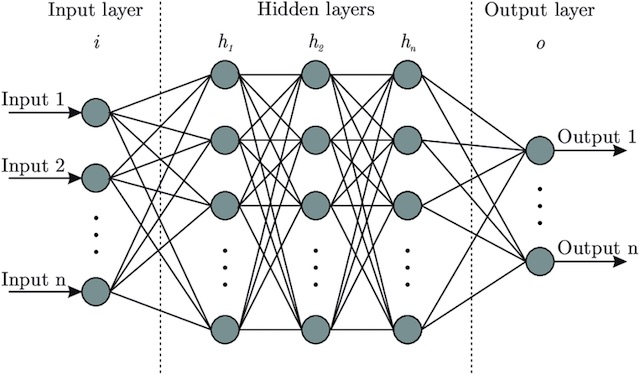
\includegraphics[width=0.6\linewidth]{images/MLP} 

}

\caption{Schematic diagram of a multilayer perceptron}\label{fig:mlp_schema}
\end{figure}

~

Every neural network has an input layer, which consists of one or more
nodes. This number is determined from the training data and tells us how
many features should be delivered to the neural network. In the case of
Ethereum (ETH) prices, we could use today's price and the prices of the
last 10 days (lags 1-10), so the input layer would consist of 11 nodes.
Some configurations also require a bias term to adjust the output along
with the weighted sum, which is also added to the input layer. Similarly
to the input layer, each neural network has exactly one output layer.
This can consist of one or more nodes. In this thesis, MLP is used as a
regressor and therefore only one neuron is needed in this layer.

In between are the hidden layers, whose number and size can be
configured as desired. The challenge is to find an optimal and efficient
configuration without causing overfitting of the training data. The
number of hidden layers depends primarily on the application area of the
neural network. For example, working with image recognition would
require more layers since the image file is broken down into individual
pixels. Subsequently, the layers are used to optimize from rough
outlines to the smallest detail. In our research, we came across several
methods or `rules of thumb' to optimize the model. A frequently
suggested method is explained by Andrej Karpathy (director of the AI
department of Tesla, Inc.). His GitHub entry recommends the approach of
starting with a model that is too large that causes overfitting.
Subsequently, the model is reduced by focusing on increasing training
loss and improving validation loss {[}3{]}.

The feedforward neural network used in this paper is implemented using
the R package `neuralnet'.

\hypertarget{RNN}{%
\subsubsection{2.2. Recurrent neural networks (RNN)}\label{RNN}}

Recurrent neural networks (RNN) are a further development of
conventional neural networks. While MLP use new inputs \(x_i\) in each
epoch, RNN also use sequential data \(h_i\) in addition to \(x_i\). This
sequential data are called hidden states and result from the previous
runs. This has the advantage that historical information stemming from
past predictions is included for the prediction for \(t+1\). This effect
can be intuitively explained by an example in which the flight path of a
scheduled flight is predicted using RNN. When predicting the exact
location (coordinates) of a plane, it is of great advantage to know the
location at \(t-1\) and to derive the flight direction from it. With the
inclusion of this information, the target area can be narrowed down,
which optimally leads to more accurate results. The same principle is
used in applications like machine translation and speech recognition,
where the result (here possibly letter or word) of the last epoch plays
a big role for the next prediction {[}4{]}.

~

\begin{figure}

{\centering 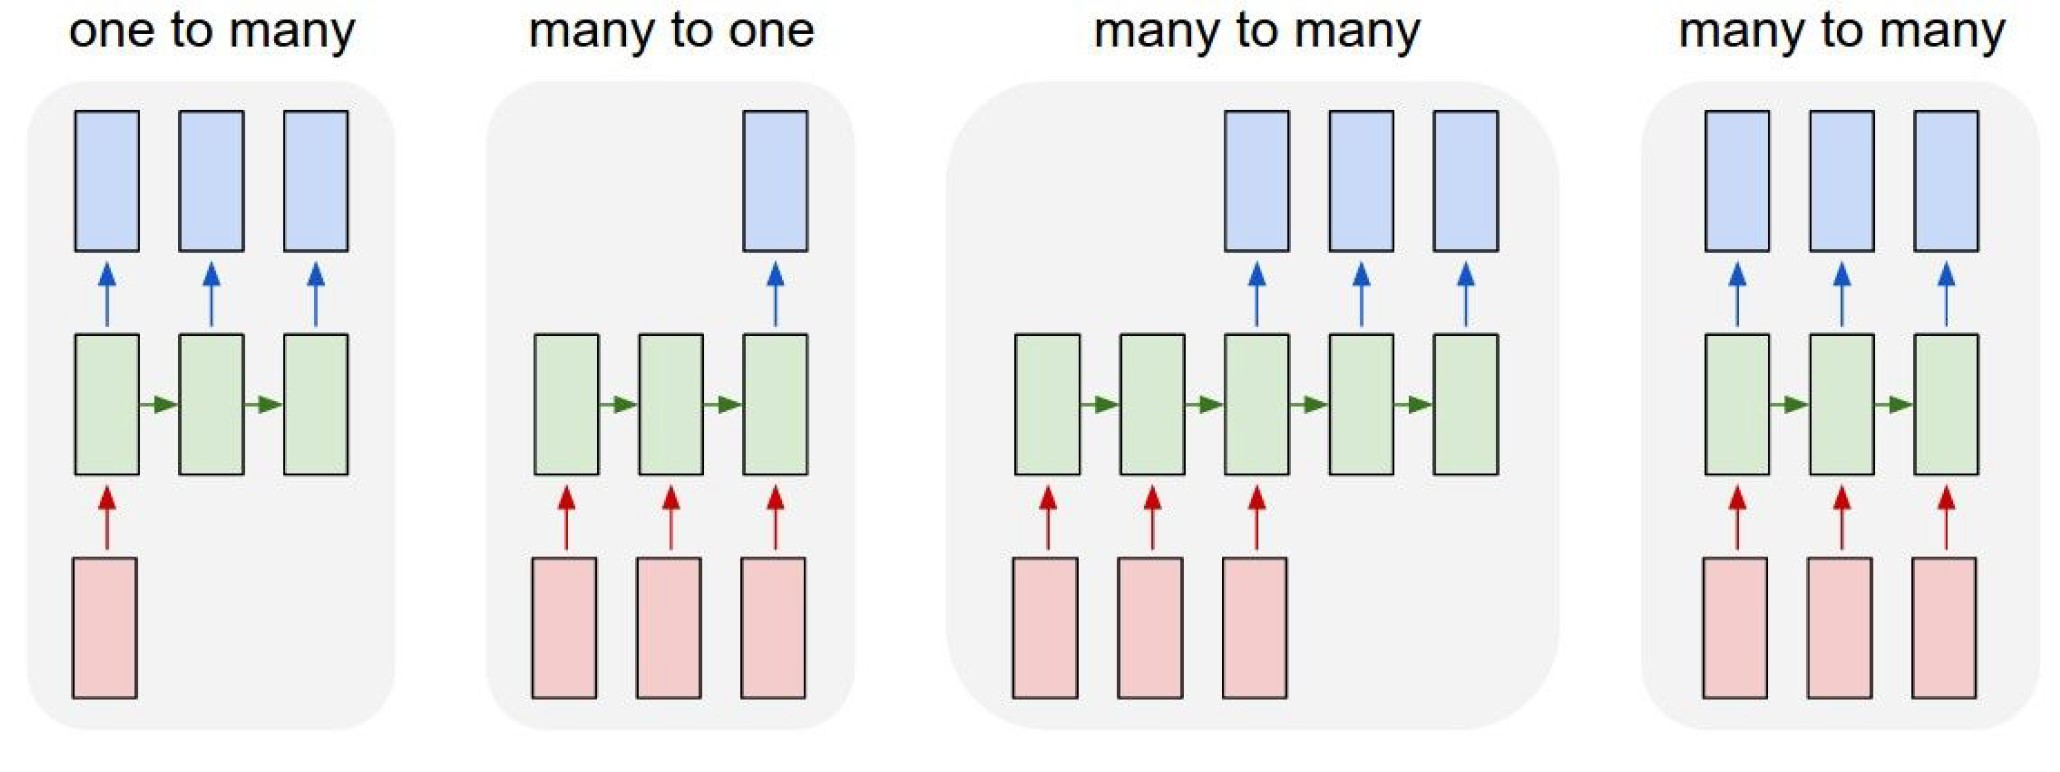
\includegraphics[width=0.8\linewidth]{images/RNN} 

}

\caption{Process sequences of different applicances of RNN.}\label{fig:RNN}
\end{figure}

~

Figure \ref{fig:RNN} shows different process sequences of the RNN, which
vary depending on the field of application. The red rectangles at the
bottom represent the number of inputs. Similarly, the blue rectangles
represent the outputs that come out of the RNN. The term `many' refers
to \(>1\) and is illustrated with three rectangles in the figure. The
green ones represent the hidden states \(h_i\) of all time steps and
thus can be seen as the memory of the neural network. The green arrows
show that the previous hidden state is used as input for the current
step. Starting from the left: one-to-many can be used for image
captioning (extracting sequence of words from images), many-to-one for
sentiment classification from sequence of words, many-to-many for
machine translation (sequence of words in one language to sequence of
words in another language) and many-to-many for video classification on
frame level {[}5{]}. For the prediction of the ETH/USD exchange rate in
this paper, we deal with the process many-to-one. This method combines
information from inputs and hidden states into one single prediction
value.

\begin{figure}

{\centering 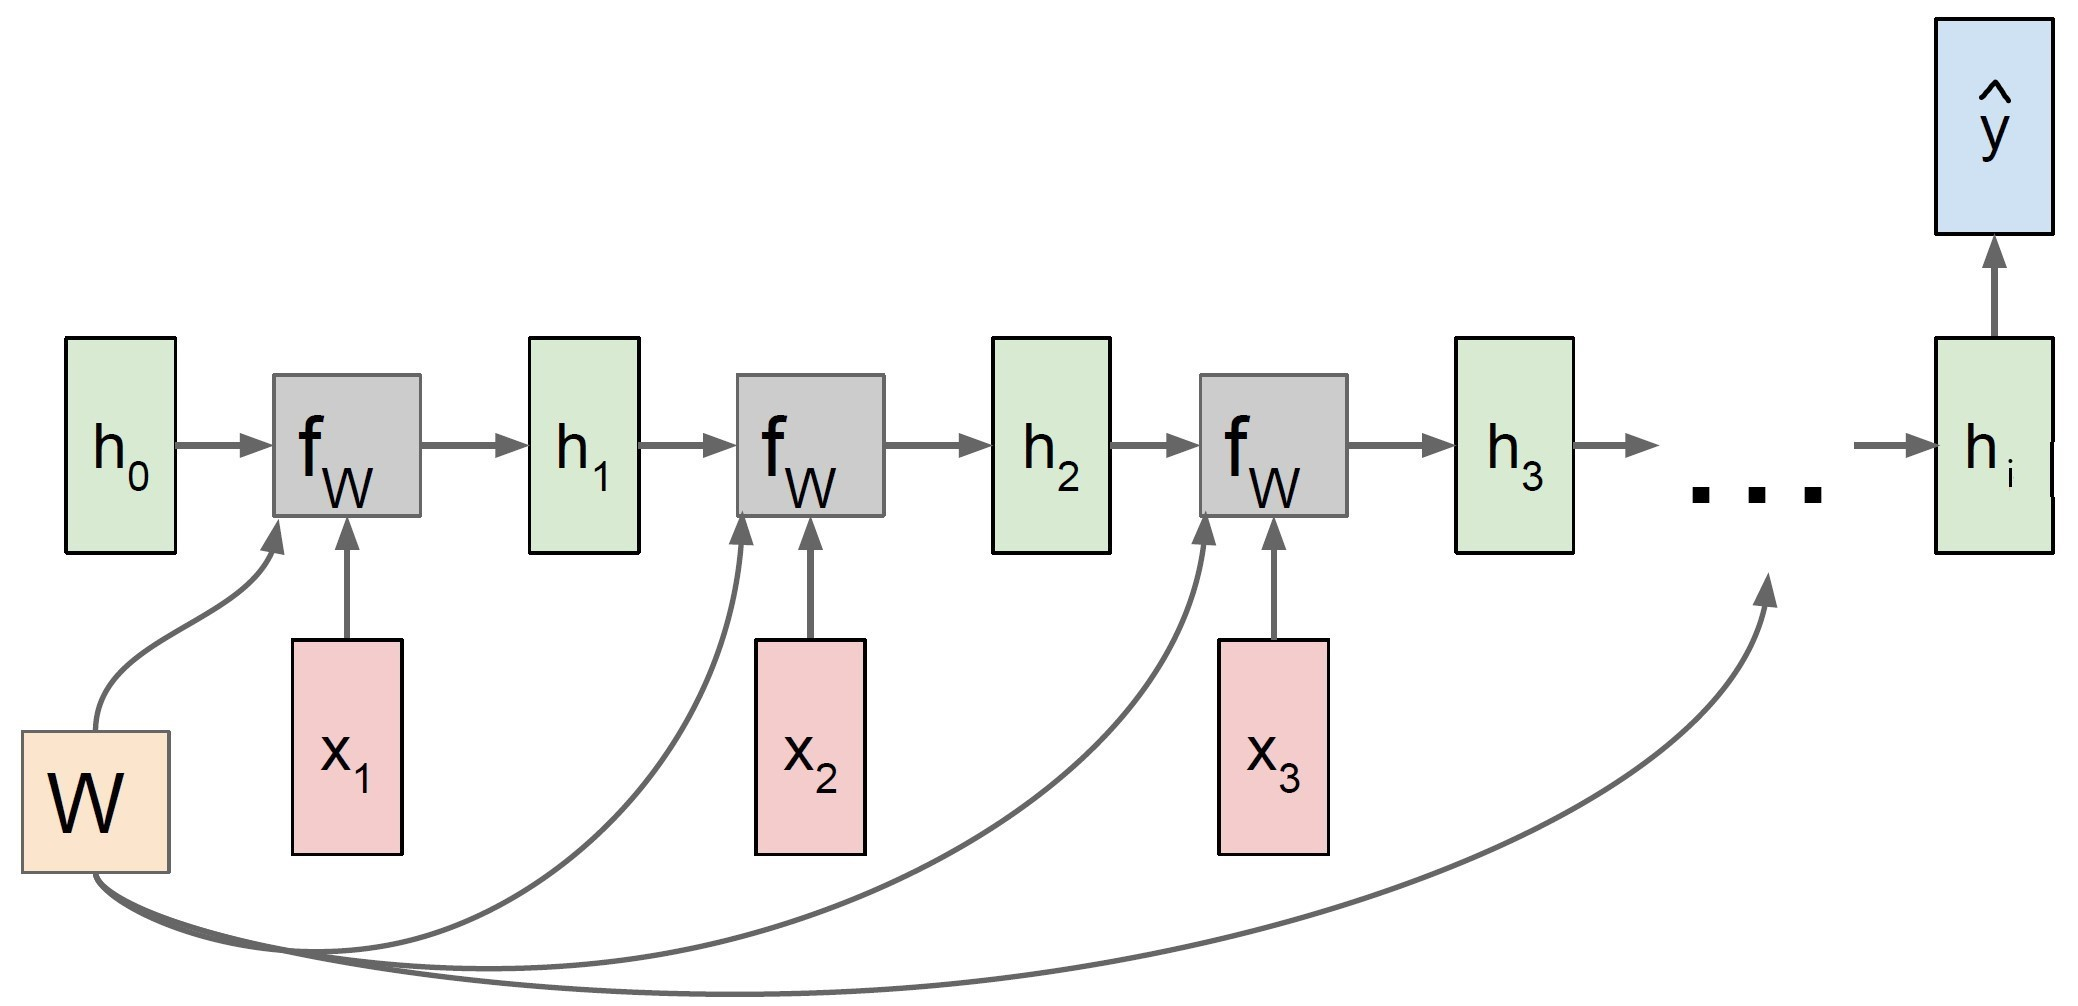
\includegraphics[width=0.7\linewidth]{images/RNN_many_to_one} 

}

\caption{Computational graph of a many-to-one RNN.}\label{fig:RNN_many_to_one}
\end{figure}

\begin{align} \label{eq:RNN_many_to_one_1}
  h_{i} & = f_{W}(h_{i-1}, x_{i}) \\
  & = \tanh(W_{h}h_{i-1} + W_{x}x_{i} + b) \nonumber 
\end{align}

Equation \ref{eq:RNN_many_to_one_1} shows how the hidden states
\(h_{i}\) are calculated at each time step, \(i\) where \(f_{W}\) is an
activation function (here: hyperbolic tangent function), \(h_{i-1}\) is
the previous state and \(x_i\) is the input vector at time step i. In
some cases, a bias term \(b\) is added to the parameters. \(W_{h}\)
represents the weight matrix for \(h_{i}\) with dimension
(length(\(h\))\(\times\)length(\(h\))). Thus, \(W_{x}\) is the weight
matrix for \(x_{i}\) with dimension
(length(\(h\))\(\times\)length(\(x\))).

\begin{align} \label{eq:RNN_many_to_one_2}
  \hat{y_{i}} = W_{y}h_{i}
\end{align}

Looking at equation \ref{eq:RNN_many_to_one_2}, \(y_{i}\) equals the
output and desired prediction of the RNN. The prediction results from
the matrix-vector product of the weight matrix \(W_{y}\) with dimension
(length(\(h\))\(\times\)length(\(y\))) and the hidden states vector
\(h\).

\newpage

\hypertarget{gated-recurrent-unit-gru-and-long-short-term-memory-lstm}{%
\subsubsection{2.3. Gated Recurrent Unit (GRU) and Long Short-Term
Memory
(LSTM)}\label{gated-recurrent-unit-gru-and-long-short-term-memory-lstm}}

In summary, recurrent neural networks retain information in memory over
time. However, it can be difficult to train standard RNN's to solve
problems that require learning long-term dependencies. This is because
the gradient of the loss function decreases exponentially with time
(vanishing gradient problem). Since the hidden states are overwritten
with many time steps, the extensions LSTM and GRU apply an extended
concept with separate memory. The weighting functions (the so-called
gates) control which information is kept and which may be forgotten.

In the GRU cell, the two gates \(r_t\) and \(z_t\) are implemented, as
can be seen in figure \ref{fig:GRU_LSTM}. Both are weighting functions
that influence whether the cell state \(s\) should be updated or the
last value is important enough to be kept. The reset gate \(r_t\)
decides if the previous hidden state \(s_{t-1}\) should be ignored. The
update gate \(z_t\) on the other hand decides if the \(\tilde{s_t}\)
should be passed to the next hidden state \(s_t\) {[}6{]}.

\begin{figure}

{\centering 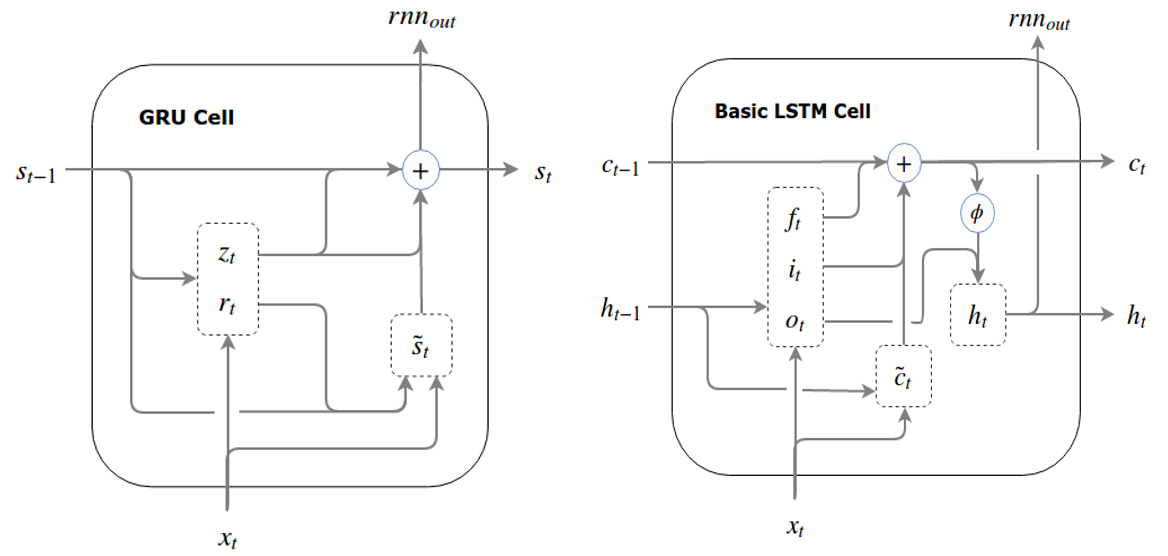
\includegraphics[width=0.9\linewidth]{images/GRU_LSTM} 

}

\caption{Workflow of a GRU cell (left) and LSTM cell (right).}\label{fig:GRU_LSTM}
\end{figure}

In contrast to the GRU cell, the LSTM cell has additional gates. They
are used to control when information enters memory, when it is output,
and when it is forgotten. This architecture allows them to learn
longer-term dependencies. The input gate \(i_t\) takes in new
information \(x_t\) and the previous hidden state \(h_{t-1}\). The
forget gate \(f_t\) gets the same information as input and controls how
much information should be kept up to which value. Information from the
previous cell state \(c_{t-1}\), the forget gate \(f_t\), the input gate
\(i_t\) and \(\tilde{c_t}\) are passed on to the next cell state
\(c_t\). Finally, the output gate \(o_t\) influences the next hidden
state \(h_t\) as well as the output of the cell {[}6{]}.

The three recurrent neural networks presented are implemented using the
R package \texttt{rnn}.

\newpage

\hypertarget{methods}{%
\subsection{3. Methods}\label{methods}}

This section covers how to define a trading strategy from the trained
networks. It is also dedicated to the topic of how the performance is
evaluated.

\hypertarget{data-exploration}{%
\subsubsection{3.1. Data exploration}\label{data-exploration}}

First, we will explore the the development of ETH over time. Figure
\ref{fig:eth_exploration} shows the price, the logarithmic price and the
log return. The logarithmic price is used to better compare the changes
from the price as the relative change becomes visible. The same is true
for the log return which shows stationarity. In the first two plots the
local peaks are well visible, which reached a then ATH (All-Time High)
of USD 1313 in January 2018. It can also be seen that we are in a bull
run at the time of writing this paper. In the log return, it can be seen
that the volatility is not constant and thus shows volatility clusters.

\begin{figure}

{\centering \includegraphics[width=0.9\linewidth]{00_main_files/figure-latex/eth_exploration-1} 

}

\caption{Time plot of the price, logarithmized price and log return based on the price for ETH/USD. Large (crypto) market phase dependencies and volatility persistence are evident.}\label{fig:eth_exploration}
\end{figure}

\newpage

Continuing with the autocorrelation (ACF) and partial autocorrelation
(PACF), we notice a dependency structure in both cases. The ACF plot in
figure \ref{fig:dependency} show that lags 5, 10, 16, 17 and 19 are
significantly stronger than just white noise. Similarly, lags 5, 10, 16,
17 and 19 are significant in the PACF plot. This information should be
kept in mind when choosing the optimal network architecture of the
neural network as it seemingly makes sense to include enough data
points.

\begin{figure}

{\centering \includegraphics[width=0.9\linewidth]{00_main_files/figure-latex/dependency-1} 

}

\caption{Autocorrelation and partial autocorrelation of log return of the ETH/USD-Prices.}\label{fig:dependency}
\end{figure}

Optimization of the ETH log return with the \texttt{auto.arima} function
from the package \texttt{forecast} indicates that it could be modeled by
an ARMA(3,3). However, occasional volatility clustering of the
standardized residuals may suggest that model assumptions for the error
term (white noise) are possibly violated. Since we are working with
neural networks, we will deal with the network architecture next.

\newpage

\hypertarget{neural-network-architecture}{%
\subsubsection{3.1. Neural Network
Architecture}\label{neural-network-architecture}}

We would like to trade ETH/USD, which is why a trustworthy forecast is
desired. Now there are countless ways how to modify neural networks and
get different solutions at best. In order to reduce the scope, we limit
ourselves to a 6-month in-sample and a 1-month out-of-sample split.
First, this shortens the computational work and we can compare different
methods and architectures using the same time period. In addition, the
split is proposed in {[}7{]}. The split can be seen in figure
\ref{fig:limit}, where red is the in-sample and blue is the
out-of-sample. The autocorrelation function of the datasubset shows
dependence at lag 5 and 10, which is why we go to a maximum of lag 10
for the input layer.

In addition, we limit ourselves in terms of network architecture. On the
one hand, the added value for too large networks is somewhat moderate
for time series (source) and on the other hand, this would go beyond the
scope of this work. For each network type presented in section
\protect\hyperlink{theory}{2}, network architectures from 1 layer with 1
neuron to 3 layers with 10 neurons each are trained. We thus examine a
total of 1100 different neuron layer combinations, with (1) the simplest
and (10,10,10) the most complex network. To make a comparison possible,
the respective in/out-of sample MSEs and Sharpe ratios are calculated
for each network. To mitigate the problem of optimizing the
backpropagation algorithm, 100 nets are trained and averaged for each
architecture for the feedforward networks (FFN). For the recurrent
network types (RNN, LSTM, GRU) only 10 networks per architecture are
trained but with 10 epochs each.

\begin{figure}

{\centering \includegraphics[width=0.9\linewidth]{00_main_files/figure-latex/limit-1} 

}

\caption{Subset of 7 months. Log returns on the left, acf on the right.}\label{fig:limit}
\end{figure}

Figure \ref{fig:limit} visualizes the MSEs for in- and out-of sample of
all neuron-layer combinations for all 4 network types. The network
architectures are separated by color. On the far left in red, are the
networks with only one layer. We have only 10 networks with one layer,
which is why this area is very small. In comparison, in the purple part
are all networks with a 3-layer architecture.

\newpage

Noticeable in black are the MSE's of the FFN networks. They are very
different from the 3 recurrent types. One can see strongly how the
network architecture influences the error terms. With increasing
complexity, the error in the in-sample decreases but increases in the
out-of-sample. This indicates an overfitting of the backpropagation
algorithm. It is curious how from a rather small MSE with architecture
(10,10) with 2-layers, to the change to the 3-layer architecture with
only one neuron each (1,1,1), the MSE makes a jump upwards. Despite the
extension to 3 layers, the number of neurons is smaller and leads to a
more stable solution.

\begin{figure}

{\centering \includegraphics[width=0.9\linewidth]{00_main_files/figure-latex/meanplot1-1} 

}

\caption{In and out-of sample MSE of all neural networks. For FFN, 100 networks were averaged in each case. For the recurrent ones, only 10 were averaged.}\label{fig:meanplot1}
\end{figure}

It is difficult to determine an optimal architecture based on the MSE.
Simply taking the smallest value would not be effective. Small in-sample
MSE values appear with complex networks, which tend to overfitting
out-of-sample. Additionally, the 3 recurrent types are visualized. You
can hardly distinguish them from each other in this figure.
Nevertheless, you can see how all 3 varies around a fixed value. For a
better interpretability only the RNN types are visualized in the
following figure \ref{fig:meanplot2}.

\newpage

Here you can see the structure of the recurrent networks a little
better. There is no pattern like in the FFN, the MSE's have no inverse
correlation between in and out-of sample. There is a certain value that
is not undercut. The MSE cannot get better than a certain value. The
spikes that occur uniformly are striking. An examination of the results
showed that the spikes appear with certain network architectures. If
only 1 or 2 neurons were specified in each case in the last layer, then
this leads to this strange spike. In the attachment in figure
\ref{fig:attachment1}, the neuron-layer combinations with 1 or 2 neurons
in the last layer have been removed. There you can see how the spikes
have disappeared. Keep in mind, however, that the differences between
apparent convergence and a spike are not very large. Furthermore, only
10 networks per combination were trained. This structure could possibly
look weakened if one would increase the number of networks.

~

\begin{figure}

{\centering \includegraphics[width=0.9\linewidth]{00_main_files/figure-latex/meanplot2-1} 

}

\caption{In and out-of sample MSE of the 3 different recurrent network types.}\label{fig:meanplot2}
\end{figure}

Nevertheless, we cannot use this visualization to determine an optimal
network architecture based on the MSE. Regardless of the complexity, one
achieves approximately the same error.

\newpage

\begin{figure}

{\centering \includegraphics[width=0.9\linewidth]{00_main_files/figure-latex/sharpeplot-1} 

}

\caption{In and out-of sample Sharpe ratios of all neural networks.}\label{fig:sharpeplot}
\end{figure}

\newpage

The architecture which we previously defined, are now used to compare
against each other. Due to the random component in all the nets we chose
a minimum of 100 nets to find an appropriate average.

This procedure is done for ffn, gru, lstm and also rnn. The results for
each net can be found in the
\protect\hyperlink{attachement}{attachement}.

In figure \ref{fig:ffn} the average performance for ffn is visualized in
red and the benchmark ``buy and hold'' is in black. Notable is for the
most nets, the performance is above zero, that might be due to the
strong upward trend in the data. For an longer out of sample, the
distribution of the N nets around the mean, would most likely look more
symmetric than it does for only this 30-day out of sample.

For the GRU LSTM and RNN (plots in
\protect\hyperlink{attachement}{attachement}) nets performance seems
similar as seen in figure \ref{fig:sharpeplot} converging to buy and
hold.

\begin{itemize}
\tightlist
\item
  FFN (1, 4)
\item
  RNN (7)
\item
  LSTM (9, 8, 2)
\item
  GRU (8, 9)
\end{itemize}

\begin{figure}

{\centering \includegraphics[width=0.9\linewidth]{00_main_files/figure-latex/ffn-1} 

}

\caption{FF out of sample}\label{fig:ffn}
\end{figure}

\newpage

\hypertarget{results}{%
\subsection{4. Results}\label{results}}

When all 4 nets are compared against Buy and Hold in figure
\ref{fig:performance}, we observe that the feed forward net performs
slightly better than buy and hold ,whilst the other 3 nets are not
better or even equal. When we look closer the decision of feedforward in
(Letter A \ref{fig:performance}) is crucial to the performance. Further
the decision in (Letter B \ref{fig:performance}) almost brought the
performance back to buy and hold.

From this Behavior it is clear that the benefit in the performance is
random.

\begin{figure}

{\centering \includegraphics[width=0.9\linewidth]{00_main_files/figure-latex/performance-1} 

}

\caption{Performance all}\label{fig:performance}
\end{figure}

\newpage

\hypertarget{conclusion}{%
\subsection{5. Conclusion}\label{conclusion}}

In recapitulation of the results we conclude that RNN GRU and LSTM bring
no further Benefit in forecasting of financial timeseries.

\newpage

\hypertarget{references}{%
\subsection{6. References}\label{references}}

\hypertarget{refs}{}
\begin{cslreferences}
\leavevmode\hypertarget{ref-perceptron_paper}{}%
{[}1{]} F. Rosenblatt, \emph{The perceptron: A probabilistic model for
information storage and organization in the brain}. Psychological
Review, 1958, pp. 386--408.

\leavevmode\hypertarget{ref-mlp_architecture}{}%
{[}2{]} M. A. J. I. Hassan Ramchoun Youssef Ghanou, \emph{Multilayer
perceptron: Architecture optimization and training}. International
Journal of Interactive Multimedia; Artificial Intelligence, 2016, p. 26.

\leavevmode\hypertarget{ref-recipe_training}{}%
{[}3{]} A. Karpathy, ``A recipe for training neural networks.''
\url{https://karpathy.github.io/2019/04/25/recipe/} (accessed Mar. 24,
2021).

\leavevmode\hypertarget{ref-RNN}{}%
{[}4{]} M. N. S. S. Ke-Lin Du, \emph{Recurrent neural networks}.
Springer London, 2014, pp. 337--353.

\leavevmode\hypertarget{ref-RNN_Stanford}{}%
{[}5{]} S. Y. Fei-Fei Li Justin Johnson, \emph{Lecture 10: Recurrent
neural networks}. Stanford University, 2017.

\leavevmode\hypertarget{ref-GRU_LSTM}{}%
{[}6{]} R2RT, ``Written memories: Understanding, deriving and extending
the lstm.''
\url{https://r2rt.com/written-memories-understanding-deriving-and-extending-the-lstm.html}
(accessed 2021).

\leavevmode\hypertarget{ref-nnfin}{}%
{[}7{]} R. R. Georgios Sermpinis Andreas Karathanasopoulos, \emph{Neural
networks in financial trading}. online: Springer Science+Business Media,
2019, p. 16.
\end{cslreferences}

\textless\textless\textless\textless\textless\textless\textless{} HEAD
\newpage

\hypertarget{attachement}{%
\subsection{7.1. Attachment}\label{attachement}}

This work is created with R-4.0.2 , RStudio Version 1.4.904 and
RMarkdown in collaborative working via Git / Github
\url{https://github.com/majimaken/econometrics-3-project}

\begin{figure}

{\centering \includegraphics[width=0.9\linewidth]{00_main_files/figure-latex/LSTM-1} 

}

\caption{GRU out of sample}\label{fig:LSTM}
\end{figure}

\begin{figure}

{\centering \includegraphics[width=0.9\linewidth]{00_main_files/figure-latex/rnn-1} 

}

\caption{RNN out of sample}\label{fig:rnn}
\end{figure}

\begin{figure}

{\centering \includegraphics[width=0.9\linewidth]{00_main_files/figure-latex/gru-1} 

}

\caption{GRU out of sample}\label{fig:gru}
\end{figure}

=======

\newpage

\hypertarget{attachment}{%
\subsection{Attachment}\label{attachment}}

\begin{figure}

{\centering \includegraphics[width=0.9\linewidth]{00_main_files/figure-latex/attachment1-1} 

}

\caption{The upper plot shows the original values. In the lower plot, the values with 1 or 2 neurons in the last layer have been removed.}\label{fig:attachment1}
\end{figure}

\begin{quote}
\begin{quote}
\begin{quote}
\begin{quote}
\begin{quote}
\begin{quote}
\begin{quote}
main
\end{quote}
\end{quote}
\end{quote}
\end{quote}
\end{quote}
\end{quote}
\end{quote}

\end{document}
